% ŠABLONA PRO PSANÍ ZÁVĚREČNÉ STUDIJNÍ PRÁCE
%%%%%%%%%%%%%%%%%%%%%%%%%%%%%%%%%%%%%%%%%%%%
% Autor: Jakub Dokulil (kubadokulil99@gmail.com)
% Tato šablona byla vytvořena tak, aby pomocí ní mohli v systému LaTeX soutěžící sázet své práce a zároveň odpovídala požadavkům na formátování vyplývajícím z wordové šablony umístěné na webu soc.cz.
%
\documentclass[12pt, a4paper,
%oneside,      %% -- odkomentujte, pokud chcete svou práci mít pouze jednostrannou, mezera pro hřbet pak automaticky bude pouze na levé straně
twoside,        %% -- pro oboustranné práce, mezera pro hřbet následně střídá strany.
openright
]{report}

%% Nutné balíčky a nastavení
%%%%%%%%%%%%%%%%%%%%%%%%%%%%

%% Proměnné
\newcommand\obor{INFORMAČNÍ TECHNOLOGIE} %% -- napiš číslo a název tvého oboru
\newcommand\kodOboru{18-20-M/01} %% -- napiš číslo a název tvého oboru
\newcommand\zamereni{se zaměřením na počítačové sítě a programování} %% -- napiš číslo a název tvého oboru
\newcommand\skola{Střední škola průmyslová a umělecká, Opava} %% vyplň název školy
\newcommand\trida{IT4} %% vyplň jméno svého konzultanta
\newcommand\jmenoAutora{Lukáš Kanovský}  %% vyplň své jméno
\newcommand\skolniRok{2023/24} %% vyplň rok
\newcommand\datumOdevzdani{1. 1. 2024} %% vyplň rok
\newcommand\nazevPrace{StrojkaVR} %% vyplň název své práce


\title{\nazevPrace} %% -- Název tvé práce
\author{\jmenoAutora} %% -- tvé jméno
\date{\datumOdevzdani} %% -- rok

\usepackage[top=2.5cm, bottom=2.5cm, left=3.5cm, right=1.5cm]{geometry} %% nastaví okraje, left -- vnitřní okraj, right -- vnější okraj

\usepackage[czech]{babel} %% balík babel pro sazbu v češtině
\usepackage[utf8]{inputenc} %% balíky pro kódování textu
\usepackage[T1]{fontenc}
\usepackage{cmap} %% balíček zajišťující, že vytvořené PDF bude prohledávatelné a kopírovatelné

\usepackage{graphicx} %% balík pro vkládání obrázků

\usepackage{subcaption} %% balíček pro vkládání podobrázků
\usepackage{float}
\usepackage{hyperref} %% balíček, který v PDF vytváří odkazy

\linespread{1.25} %% řádkování
\setlength{\parskip}{0.5em} %% odsazení mezi odstavci


\usepackage[pagestyles]{titlesec} %% balíček pro úpravu stylu kapitol a sekcí
\titleformat{\chapter}[block]{\scshape\bfseries\LARGE}{\thechapter}{10pt}{\vspace{0pt}}[\vspace{-22pt}]
\titleformat{\section}[block]{\scshape\bfseries\Large}{\thesection}{10pt}{\vspace{0pt}}
\titleformat{\subsection}[block]{\bfseries\large}{\thesubsection}{10pt}{\vspace{0pt}}


\usepackage{tocloft} % Balíček umožní přizpůsobit vzhled tabulky obsahu
\setlength{\cftbeforechapskip}{0pt}  % Menší rozestup pro kapitoly
\setlength{\cftbeforesecskip}{0pt}   % Menší rozestup pro sekce

\setcounter{secnumdepth}{2}
\setcounter{tocdepth}{1}
\usepackage{fancyhdr}
\pagestyle{fancy}
\fancyhf{}
\renewcommand{\headrulewidth}{0pt}
\fancyfoot[C]{\thepage}



\usepackage{booktabs}

\usepackage{url}

%% Balíčky co se můžou hodit :) 
%%%%%%%%%%%%%%%%%%%%%%%%%%%%%%%

\usepackage{pdfpages} %% Balíček umožňující vkládat stránky z PDF souborů, 

\usepackage{upgreek} %% Balíček pro sazbu stojatých řeckých písmen, třeba u jednotky mikrometr. Například stojaté mí: \upmu, stojaté pí: \uppi

\usepackage{amsmath}    %% Balíčky amsmath a amsfonts 
\usepackage{amsfonts}   %% pro sazbu matematických symbolů
\usepackage{esint}     %% pro sazbu různých integrálů (např \oiint)
\usepackage{mathrsfs}
\usepackage{helvet} % Helvet font
\usepackage{mathptmx} % Times New Roman
\usepackage{Oswald} % Oswald font


%% makra pro sazbu matematiky
\newcommand{\dif}{\mathrm{d}} %% makro pro sazbu diferenciálu, místo toho
%% abych musel psát '\mathrm{d}' mi stačí napsat '\dif' což je mnohem 
%% kratší a mohu si tak usnadnit práci

\let\oldchapter\chapter
\renewcommand{\chapter}{
	\clearpage
	\pagestyle{fancy}
	\oldchapter
}

\usepackage{listings}
\usepackage{xcolor}

\renewcommand{\lstlistingname}{Kód}% Listing -> Algorithm
\renewcommand{\lstlistlistingname}{Seznam programových kódů}% List of Listings -> List of Algorithms


%copied code start
\definecolor{mediumgray}{rgb}{0.3, 0.4, 0.4}
\definecolor{mediumblue}{rgb}{0.0, 0.0, 0.8}
\definecolor{forestgreen}{rgb}{0.13, 0.55, 0.13}
\definecolor{darkviolet}{rgb}{0.58, 0.0, 0.83}
\definecolor{royalblue}{rgb}{0.25, 0.41, 0.88}
\definecolor{crimson}{rgb}{0.86, 0.8, 0.24}

\lstdefinestyle{csh}{
	language=C,
	backgroundcolor=\color{white},
	basicstyle=\ttfamily,
	breakatwhitespace=false,
	breaklines=false,
	captionpos=b,
	columns=fullflexible,
	commentstyle=\color{mediumgray}\upshape,
	emph={},
	emphstyle=\color{crimson},
	extendedchars=true,  % requires inputenc
	fontadjust=true,
	frame=single,
	identifierstyle=\color{black},
	keepspaces=true,
	keywordstyle=\color{mediumblue},
	keywordstyle={[2]\color{darkviolet}},
	keywordstyle={[3]\color{royalblue}},
	literate=%
	{á}{{\'a}}1 {č}{{\v{c}}}1 {ď}{{\v{d}}}1 {é}{{\'e}}1 {ě}{{\v{e}}}1
	{í}{{\'i}}1 {ň}{{\v{n}}}1 {ó}{{\'o}}1 {ř}{{\v{r}}}1 {š}{{\v{s}}}1
	{ť}{{\v{t}}}1 {ú}{{\'u}}1 {ů}{{\r{u}}}1 {ý}{{\'y}}1 {ž}{{\v{z}}}1,		
	numbers=left,
	numbersep=5pt,
	numberstyle=\tiny\color{black},
	rulecolor=\color{black},
	showlines=true,
	showspaces=false,
	showstringspaces=false,
	showtabs=false,
	stringstyle=\color{forestgreen},
	tabsize=2,
	title=\lstname,
	upquote=true  % requires textcomp	
}
% copied code end






%% Bordel pro práci - můžeš smáznout :) 
%%%%%%%%%%%%%%%%%%%

\usepackage{lipsum} %% balíček který píše lipsum (nesmyslný text, který se používá pro kontrolu typografie)

%% Začátek dokumentu
%%%%%%%%%%%%%%%%%%%%
\begin{document}
	
	\pagestyle{empty}
	\pagenumbering{Roman}
	
	\cleardoublepage

%% Titulní stránka s informacemi
%%%%%%%%%%%%%%%%%%%%%%%%%%%%%%%%%%%%%%%%
	
	{\fontfamily{phv}\selectfont
		%% Logo školy
		\begin{figure}[h]
			\centering
			
\includegraphics[width=0.6\linewidth]{image/logo-skoly.png} 
		\end{figure}
		
		
		%% Hlavička práce a její název (viz proměnná \nazev prace)
		%% \sffamily %%% bezpatkové písmo - sans serif
		{\bfseries %%% písmo na stránce je tučně
			\begin{center}
				\vspace{0.025 \textheight}
				\LARGE{ZÁVĚREČNÁ STUDIJNÍ PRÁCE}\\
				\large{dokumentace}\\
				\vspace{0.075 \textheight}
				\LARGE {\nazevPrace}\\
			\end{center}  
		}%%%
		
		\begin{figure}[h]
			\centering
			
\includegraphics[width=0.5\linewidth]{image/logo.png} 
		\end{figure}
		
		\vspace{0.02 \textheight}
		\begin{table}[h!]
			\begin{tabular}{ll}
				\textbf{Autor:} & \jmenoAutora\\ 
				\textbf{Obor:} & \kodOboru { } \obor\\
				\textbf{} & \zamereni\\
				\textbf{Třída:} & \trida\\
				\textbf{Školní rok:} & \skolniRok\\
			\end{tabular}
			
		\end{table}		
	}
	
%% Stránka obsahující poděkování 
%%%%%%%%%%%%%%%%%%%%%%%%%%%%%%%%%%%%%%%%%%%%%%%%%%%%%%%%

%% Poděkování - nepovinné
%%%%%%%%%%%%%%%%%%%%%%%%%%%%
	\noindent{\large{\bfseries{Poděkování}\\}}
	\noindent{Chtěl bych poděkovat Michaele Říčné za poskytnutí všech 3D modelů. Také bych rád poděkoval Beátě Muchové za design loga, uživatelského rozhraní a obrazů použitých v aplikaci.}

	
	\vspace*{0.7\textheight} %% Vertikální mezeru je možné upravit

%% Prohlášení - povinné
%%%%%%%%%%%%%%%%%%%%%%%%%%%%
	\noindent{\large{\bfseries{Prohlášení}\\}}  %% uprav si koncovky podle toho na jaký rod se cítíš, vypadá to pak lépe :) 
	\noindent{Prohlašuji, že jsem závěrečnou práci vypracoval samostatně a uvedl veškeré použité 
		informační zdroje.\\}
	\noindent{Souhlasím, aby tato studijní práce byla použita k výukovým a prezentačním účelům na Střední průmyslové a umělecké škole v Opavě, Praskova 399/8.}
	\vfill
	\noindent{V Opavě \datumOdevzdani\\}
	\noindent
	\begin{minipage}{\linewidth}
		\hspace{9.5cm} 
		\begin{tabular}{@{}p{6cm}@{}}
			\dotfill \\
			Podpis autora
		\end{tabular}
	\end{minipage}

%% Stránka obsahující abstrakt (anotaci)
%%%%%%%%%%%%%%%%%%%%%%%%%%%%%%%%%%%%%%%%%%%%%%%%%%%%%%%%	

%% Abstrakt v češtině
%%%%%%%%%%%%%%%%%%%%%%%%%%%%
	\noindent{\Large{\bfseries{Abstrakt}\\}}
Práce se zabývá tvorbou aplikace pro virtuální realitu. Také zmiňuje problematiku virtuální reality. Výsledkem práce je aplikace vytvořená v Unity. V aplikaci je udělaná jedna třída odborného předmětu. V ní jsou umístěny objekty a s určitými je možné i interagovat. Ve třídě je rozmístěno deset počítačových komponentů, mezi ně patří napájecí zdroj, SSD disk, základní deska, grafická karta, procesor, chladič na procesor a čtyři paměti RAM. Ty musí uživatel najít a poskládat do počítače, který se nachází na stole v přední části třídy. Uživatel se ovládání a cíl místnosti může dozvědět z uživatelského menu, které je umístěné na levé ruce.

	
	\vspace{18pt}
	
	\noindent{\large{\bfseries{Klíčová slova}}}
	
	\noindent Virtuální realita, Unity, Škola
	
	\vspace{18pt}

%% Abstrakt v angličtině
%%%%%%%%%%%%%%%%%%%%%%%%%%%%	
	\noindent{\Large{\bfseries{Abstract}\\}}
	The work focuses on creating an application for virtual reality, addressing issues related to virtual reality. The result of the work is an application developed in Unity. Within the application, there is a class representing a specialized subject. Objects are placed within this class, and some of them can be interacted with. The class contains ten computer components, including a power supply, SSD disk, motherboard, graphics card, processor, processor cooler, and four RAM modules. The user needs to locate and assemble these components into a computer, which is positioned on a table at the front of the class. The user can learn about the controls and the room's objective through the user menu located on the left hand.
	
	\vspace{18pt}
	
	\noindent{\large{\bfseries{Keywords}}}
	
	\noindent Virtual Reality, Unity, School
	
	\newpage

%% Stránka s generovaným obsahem
%%%%%%%%%%%%%%%%%%%%%%%%%%%%%%%%%%%%%%%	
	
	\tableofcontents %% Vygeneruje tabulku s obsahem

	\pagenumbering{arabic} %% Nastavení způsobu číslování stránek (alternativy roman | Roman)
	\setcounter{page}{1} %% Nastavení počitadla stránek

%% Stránka s úvodem - povinná část
%%%%%%%%%%%%%%%%%%%%%%%%%%%%%%%%%%%%%%%		
	\chapter*{Úvod}
	\addcontentsline{toc}{chapter}{Úvod}
	Cílem práce bylo vytvořit aplikaci pro virtuální realitu. Prvotním nápadem bylo vytvořit třídy odborných předmětů ze školy a ke každé třídě napsat popis co se v předmětu dělá a udělat modely předmětů, se kterými se v hodinách pracuje. Z tohoto nápadu jsem sešel a rozhodl jsem se udělat pro každou třídu menší interaktivní hru.
	
	Motivací pro tento projekt bylo pochopit jak funguje virtuální realita, ale také jsem se chtěl zlepšit v Unity a vytváření her či aplikací v něm.
	
	Práce popisuje co je to virtuální realita, její využití a typy. Poté popisuje průběh vytváření celé aplikace, jako je prvotní nastavení projektu v Unity. Dále tvorbu místnosti a následnému pohybu v ní. Řešení interakcí s objekty a stavění počítače.
%* náhled do řešené problematiky, zdůvodnění volby problematiky, 
%* předem definované cíle práce, 
%* motivaci pro další čtení textu včetně stručného uvedení obsahu následujících kapitol 


\chapter{Virtuální realita}

\section{Co je to virtuální realita}
\label{sec:co_je_VR}
Virtuální realita (VR) je technologie, která vytváří počítačem generované prostředí, které uživatele ponořuje do simulovaného světa. Tato technologie využívá kombinaci hardware, software a často i speciálních periférií, aby vytvořila iluzi, že uživatelé jsou přítomní a interagují s prostředím, které ve skutečnosti není fyzicky kolem nich.


\section{Využití virtuální reality}
\label{sec:vyuziti_VR}


\begin{itemize}
	\item Herní průmysl,
	\item vzdělávání,
	\item architektura a design,
	\item lékařství.
\end{itemize}


\section{Typy virtuální reality}
\label{sec:typy_VR}


\subsection{Nízká úroveň virtuální reality}
Nejedná se o plně interaktivní VR, ale o 360° videa, která pokrývají všechny směry a umožňují uživatelům pohybovat se kolem v daném prostředí. 

\subsection{Vysoká úroveň virtuální reality}
Plně interaktivní virtuální prostředí, které pomocí ovladačů umožňují uživatelům pohybovat se, interagovat s objekty a provádět různé akce.

\subsection{Pokročilá virtuální realita}
Využívá prvků smíšené reality (mixed reality - MR) což je kombinace fyzického světa s virtuální realitou, kde jsou digitální objekty integrovány do reálného prostředí.

Dále využívá rozšířené reality (augmented reality - AR), která podobně jako MR přidává digitální objekty do reálného světa, aniž by uživatel byl plně ponořen do virtuálního prostoru.

\chapter{Aplikace v Unity}	

Aplikace je vytvořena v herním enginu Unity, ve kterém můžete využít různých balíčků, šablon a assetů.

	\section{Meta Quest 2}
\label{sec:meta_quest_2}

	Meta Quest 2 je původně vyvíjený společností Oculus je VR headset s ovladači, na který jsem aplikaci vyvíjel. Meta Quest 2 používá vlastní operační systém založený na Androidu.
	
	\subsubsection{Výhody:}
	\begin{itemize}
		\item Samostatnost: Meta Quest 2 je bezdrátový, to znamená že není potřeba připojení k počítači. To poskytuje uživatelům větší volnost pohybu,
		\item vestavěný sledovač pohybu: Díky vestavěným senzorům není zapotřebí montovat do místnosti senzory, což zjednodušuje užívání headsetu,
		\item dostupnost aplikací: Meta nabízí otevřenou platformu Meta Store, kde je k dispozici široká škála her a aplikací,
		\item sociální funkce: Do headsetu si můžete propojit různé sociální sítě. To vám umožní psát nebo volat s lidmi přímo z prostředí virtuální reality.
	\end{itemize}
	
	\subsubsection{Nevýhody:}
	\begin{itemize}
		\item Omezený výkon: I přesto, že Meta Quest 2 je samostatný, jeho výkon může být omezen ve srovnání s výkonnějšími VR systémy připojenými k výkonnějším počítačům,
		\item omezený úhel sledování: Někdy může dojít k omezení sledování pohybu, zejména při pohybu rukou mimo přímý zorný úhel headsetu.
	\end{itemize}
	
	\subsection{Přidávání vlastních aplikací do Meta Quest 2:}
	Existuje více možností jak přidat vlastní aplikaci do headsetu. Můžete headset připojit pomocí kabelu k počítači a aplikaci či hru přetáhnout do souborů v headsetu. Další možností je aplikaci nahrát na App Lab, který je součástí Meta Store. Nebo aplikaci nahrát pomocí programů třetích stran. Nejpopulárnější je SideQuest, který jsem použil já. SideQuest se automaticky připojí na headset, pokud ho máte připojený k počítači pomocí kabelu nebo wifi. Aplikaci pak na headset nainstalujete z .apk souboru.
	
	\begin{figure}[h!]
		\centering 
		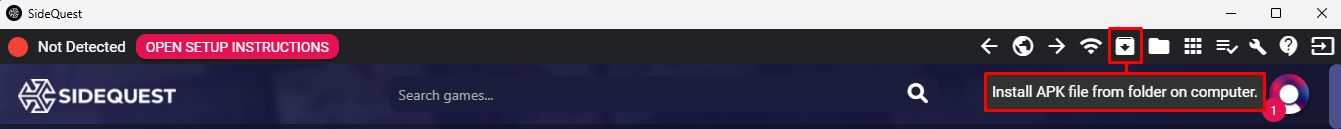
\includegraphics[width=1\textwidth]{image/sidequest.png} 
		\caption{Ukázka jak naistalovat aplikaci pomocí SideQuest.} 
		\label{fig:sidequest} 
	\end{figure}

	\section{Struktura projektu}
\label{sec:struktura_projektu}
	
	Projekt jsem rozdělil do různých složek pro přehlednost a lepší orientaci při tvorbě projektu. Složka Materials obsahuje všechny materiály či textury použité na 3D modelech. Ve složce Prefabs jsou uloženy samotné objekty importované z blenderu v souboru .fbx. Dále jsem udělal složku Scripts pro skripty, které jsem vytvořil. Další složky vytvořilo samo Unity nebo balíčky využité v projektu. 
	
		\begin{figure}[h!]
		\centering 
		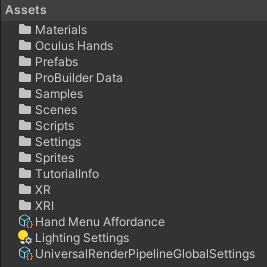
\includegraphics[width=0.4\textwidth]{image/assets.png} 
		\caption{Ukázka podsložek v projektu.} 
		\label{fig:podslozky} 
	\end{figure}
	
	\newpage
	
\section{Nastavení projektu}
\label{sec:nastaveni_projektu}
V Unity existují šablony pro různé typy projektů, které usnadní prvotní nastavení projektu. Já žádnou šablonu nepoužil, protože součástí byly věci, které bych nevyužil. Takže jsem se rozhodl prvotní incializaci a nastavení udělat sám.

Jako první jsem nastavil platformu projektu. Pro testování při tvorbě projektu jsem použil nastavení pro Windows, ale pro zkompilovaný projekt jsem použil Android, protože systém Meta Quest 2 je postavený na Androidu. Dále jsem musel nastavit XR plugin, který řídí všechny funkce pro virtuální realitu. Tam jsem nastavil OpenXR, protože podporuje širší škálu VR headsetů, na rozdíl od Oculus, který podporuje VR headsety jen od Oculusu (nyní od společnosti Meta).

Dále jsem si vytvořil základ projektu, jako XR origin, který je vlastně postava kterou ovládáte pomocí VR headsetu. Obsahuje kameru a ruce.

\begin{figure}[h!]
	\centering
	\subfloat{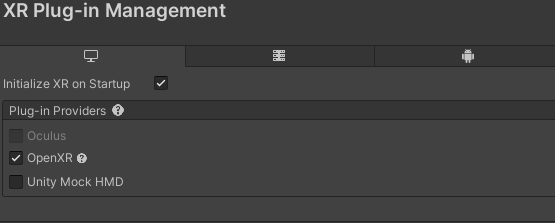
\includegraphics[width=9cm]{image/xrPluginSettings.png}}
	\qquad
	\subfloat{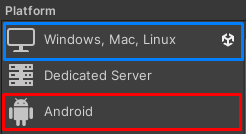
\includegraphics[width=6cm]{image/build.png}}
	\caption{Zvolení provideru pro XR plugin a platformy projektu.}
	\label{fig:nastaveni_unity}
\end{figure}


\newpage

\section {Tvorba místnosti}
\label{sec:tvorba_mistnosti}
\subsubsection{ProBuilder}
Tento balíček umožňuje stavění přímo ve scéně v Unity. Nabízí  vytváření základních geometrických tvarů, ale také vlastních složitějších tvarů. Také se v něm dají mapovat a upravovat textury. Pro samotnou manipulaci a úpravu objektů nabízí vytažení, zrcadlení, zaoblení a mnoho dalších funkcí.

\begin{figure}[H]
	\centering
	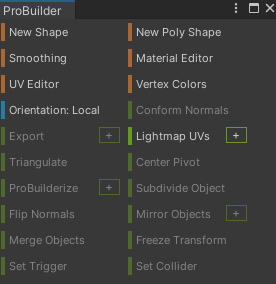
\includegraphics[width=0.4\textwidth]{image/proBuilder.png}
	\caption{Ukázka možností ProBuilderu.}
	\label{fig:ProBuilder}
\end{figure}

\subsubsection{ProGrids}
ProGrids je sice experimentální balíček, ale problémy mi sním nenastaly, takže jsem se jej rozhodl použít. V podstatě vše co tento balíček dělá je, že zachytává objekty k mřížce. To zjednodušuje tvorbu místnosti a pozdější umístění objektů do místnosti. Dá se v něm nastavit na jak velkou či malou mřížku chci přichytávat a také k jaké ose.

\begin{figure}[H]
	\centering
	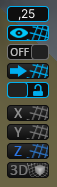
\includegraphics[width=0.1\textwidth]{image/proGrids.png}
	\caption{Ukázka ProGrids.}
	\label{fig:ProGrids}
\end{figure}

\subsubsection{Místnost}
S místností jsem se inspiroval třídou programového vybavení ve škole. Při vytváření jsem začal s kostkou, tu jsem prodloužil a protáhl ať připomíná tvar třídy. Poté jsem použil funkci inset na vrchní stranu, abych naznačil šířku zdí. To jsem poté pomocí funkce extrude protáhl dolů, aby vznikly zdi. Podlahu a strop jsem udělal jako jednoduchý plane.

Objekty jsem importoval ze souborů .fbx, ketré jsou vymodelované podle vybavení ve třídě. Objekty jsem následně umístil tak, aby byly co nejblíže reálné třídě. Všem jsem přidal collidery, tak aby co nejvěrohodněji připomínaly reálné verze objektů.

\begin{figure}[H]
	\centering
	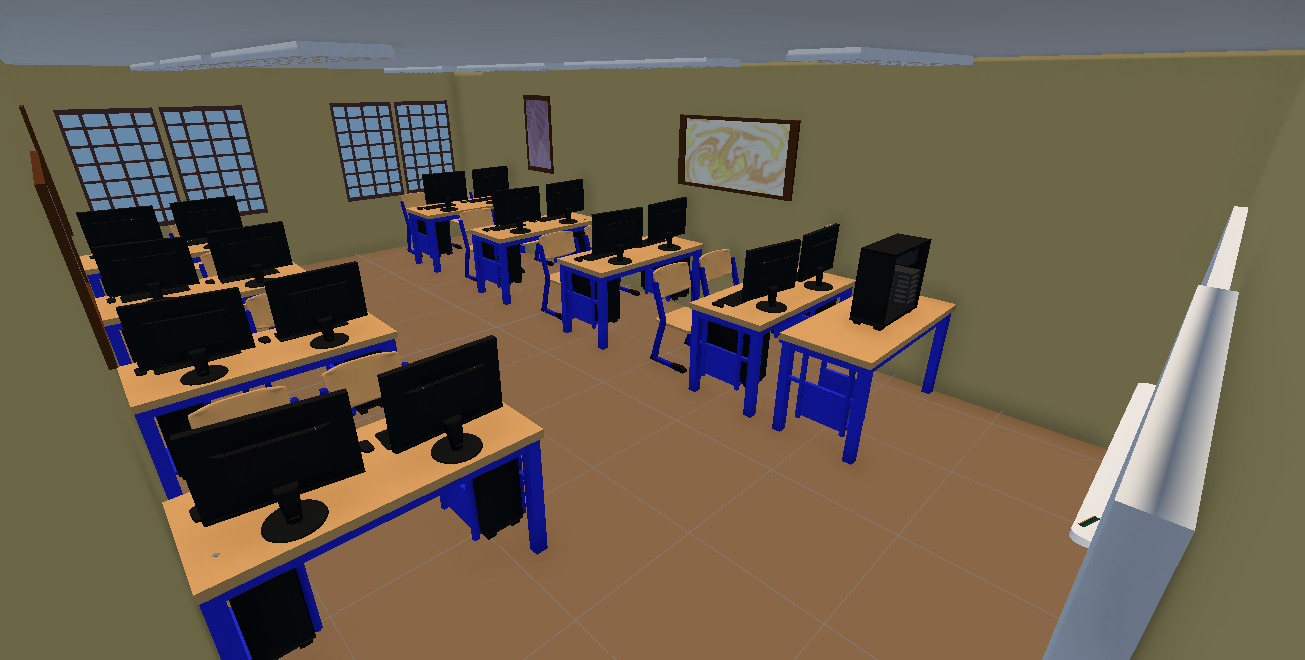
\includegraphics[width=0.9\textwidth]{image/classroom.png}
	\caption{Ukázka jak vypadá třída.}
	\label{fig:trida}
\end{figure}

\newpage

\section {Pohyb a interakce}
\label{sec:pohyb_a_interakce}
\subsection{Pohyb}
 Pohyb je řešený pomocí skriptů z XR toolkitu. Celý pohyb závisí na skriptu Locomotion System. Ten přesune reálný pohyb do virtuálního světa, ale protože pohyb po velkých virtuálních scénách by byl v realitě náročný, přidal jsem k tomu Continuous Move Provider. Díky něj můžu nastavit pohyb na joystick na jednom ze dvou ovladačů od headsetu. Já ho nastavil na levý ovladač. Dále můžu nastavit rychlost pohybu. Samozřejmě jsem myslel na otáčení, takže jsem přidal skript Continouous Turn Provider, který jsem nastavil na joystick pravého ovladače. Stejně jako při pohybu můžu nastavit rychlost otáčení.

\subsection{Interakce}
\subsubsection{Ruce}
Nejdříve než jsem mohl začít interagovat s objekty, musel jsem na nich nastavit dva skripty. První je XR Controller. Tento skript řídí všechen vstup ovladače. Druhý skript je XR Direct Interactor. Ten pro funkčnost potřebuje nějaký collider, který bude snímat, jestli koliduje s colliderem objektu, se kterým chceme interagovat. Také jsem napsal skript, který ovládá základní gesta rukou. Do skriptu se dá přidat více gest, ale více jsem jich zatím nepotřeboval.

\begin{lstlisting}[style=csh, caption={Ukázka kódu na gesta rukou.}]	
	public class VRHands : MonoBehaviour
	{
		public InputActionProperty pinchAnimationAction;
		public InputActionProperty gripAnimationAction;
		public Animator handAnimator;
		
		void Update()
		{
			float triggerValue = pinchAnimationAction.action.ReadValue<float>();
			handAnimator.SetFloat("Trigger", triggerValue);
			
			float gripValue = gripAnimationAction.action.ReadValue<float>();
			handAnimator.SetFloat("Grip", gripValue);
		}
	}
\end{lstlisting}

\subsubsection{Objekty}
Každý objekt, se kterým chci interagovat potřebuje Rigidbody. To zaručí, že objekt bude reagovat na gravitaci a bude se moct pohybovat. Ale, aby nepropadl přes podlahu nebo ostatní objekty, musí samozřejmě mít collider. Každý objekt má jiný počet colliderů, to podle jeho tvaru a stylu jakým chci, aby s ním uživatel interagoval.

Důležitý je ale skript XR Grab Interactable, který umožní objekt chytnout pomocí ovladače. Tento skript stačilo nastavit jen jednou poté nakopírovat na každý objekt, který má být uchopitelný. Skript má velikou škálu nastavení, ale pro nejlepší sledování pohybu ruky, stačilo aktivovat smooth position, rotation a přepnout typ pohybu na velocity tracking.

\begin{figure}[H]
	\centering
	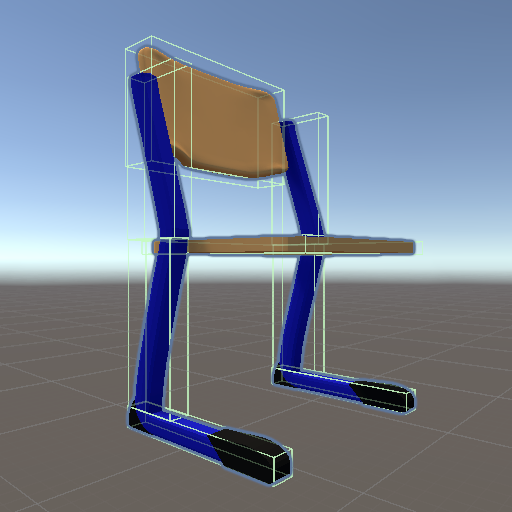
\includegraphics[width=0.5\textwidth]{image/chair.png}
	\caption{Ukázka colliderů židle.}
	\label{fig:collidery_zidle}
\end{figure}

\newpage 

\section{Uživatelské menu}
\label{sec:uzivatelske_menu}
Jako uživatelské menu jsem nechtěl dělat nic komplikovaného a složitého na pochopení nebo na navigaci. Proto jsem se rozhodl udělat jednoduché menu, které jsem umístil na levou ruku. Menu se zobrazí pouze, když se uživatel na ruku podívá.

Jakýkoliv komponent uživatelského rozhraní je řešený přes canvas (plátno). Ten je základně nastavený, že se zobrazuje jako překrytí na obrazovce. To jsem přenastavil na world space, aby bylo plátno součástí prostředí. Na plátno jsem přidal panel, který obsahuje obrázek. 

\subsubsection{Zobrazení pohledem}
Aby se menu zobrazovalo pouze, když se uživatel dívá na ruku, musel jsem přidat dva prázdné objekty. První je Gaze Interactor, ten obsahuje skript Gaze Interactor, který snímá pohled ze strany a úhlu, který jsem předem nastavil. Pod tímto úhlem se také zobrazí uživatelské menu. Druhý objekt jsem přidal na hlavní kameru, která jedná jako hlava (VR headset). Tento objekt se jmenuje Gaze Interactable. Obsahuje kulatý collider, který snímá jestli je v blízkosti Gaze Interactor. Dále má skript Simple Interactable, ten je nastavený, aby povolil interakci pohledem. Toto stačí, aby se menu zobrazovalo, když se uživatel na ruku dívá nebo schovalo, když ne.

\subsubsection{Animace zobrazení a schování menu}
Pro příjemnější a plynulejší zobrazení jsem přidal dva skripty, které ovládají průhlednost plátna. Interactable Affordance State Provider, tento skript zanimuje změnu proměnné, kterou tomu předáte. Dále jsem vytvořil Float Affordance Theme, ten jsem předal skriptu Float Affordance Receiver. Tomuto skriptu jsem nastavil, že má upravovat alfa kanál plátna.

\begin{figure}[h!]
	\centering
	\subfloat{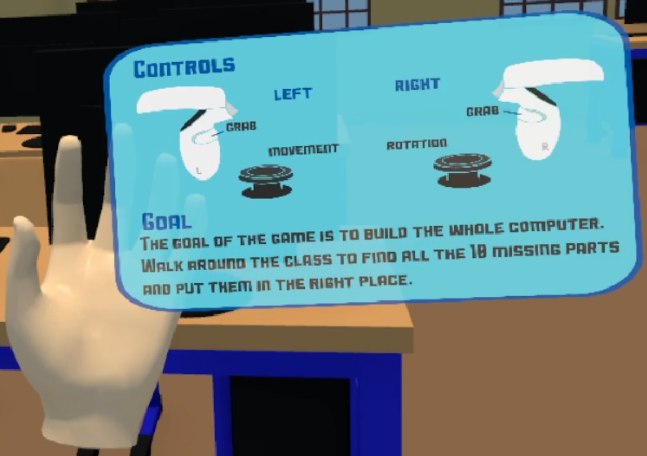
\includegraphics[width=8cm]{image/uiVisible.png}}
	\qquad
	\subfloat{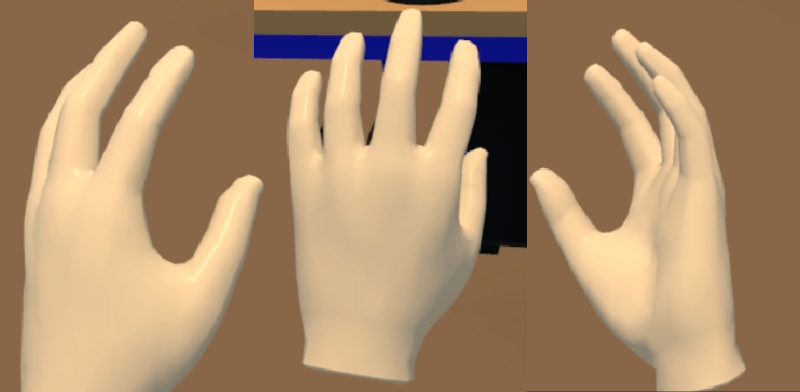
\includegraphics[width=7cm]{image/uiNotVisible.png}}
	\caption{Ukázka uživatelského menu, když jde a nejde vidět.}
	\label{fig:uzivatelske_menu}
\end{figure}

\newpage

\section{Sestavení počítače}
\label{sec:sestaveni_pocitace}
V každé třídě, která by v projektu byla, jsem chtěl udělat nějakou menší interaktivní hru. Takže jsem se rozhodl že pro tuto třídu udělám sestavení počítače.

Sestavení počítače jsem řešil pomocí skriptu Socket Interactor. S ním, ale nastaly problémy, protože jsem do počítače mohl dát jakýkoliv objekt, který lze uchopit, jako například i židle. Toto jsem spravil přidáním kontroly značky objektu, který chci do socketu dát.

Každý socket se skládá z box collideru, který je nastavený ná snímání kolize, takže tvoří jen zónu, nikoli solidní objekt. Dále má již zmíněný skript, v němž je nastavený materiál (textura), který se zobrazí když objekt vstoupí do socketu. Také jsem každému socketu nastavil značku, tak aby počítačové komponenty šly dát jen tam kam patří. A aby se komponenty položily do počítače správně, musel jsem postupně každý do počítače vložit. Otočit a posunout, tak aby se umístil jak v reálném počítači.

Když jsem se ujistil, že všechny komponenty sedí na svém místě jak mají, rozmístil jsem je různě po třídě. Uživatel musí všechny komponenty najít a poskládat do počítače.

\begin{lstlisting}[style=csh, caption={Skrip, který přidá kontrolu značky objektu.}]	
	using UnityEngine.XR.Interaction.Toolkit;
	
	public class SocketTagCheck : XRSocketInteractor
	{
		public string targetTag = string.Empty;
		
		public override bool CanHover(XRBaseInteractable interactable)
		{
			return base.CanHover(interactable) && MatchTag(interactable);
		}
		
		public override bool CanSelect(XRBaseInteractable interactable)
		{
			return base.CanSelect(interactable) && MatchTag(interactable);
		}
		
		private bool MatchTag(XRBaseInteractable interactable)
		{
			return interactable.CompareTag(targetTag);
		}
	}
\end{lstlisting}

\newpage

\begin{figure}[H]
	\centering 
	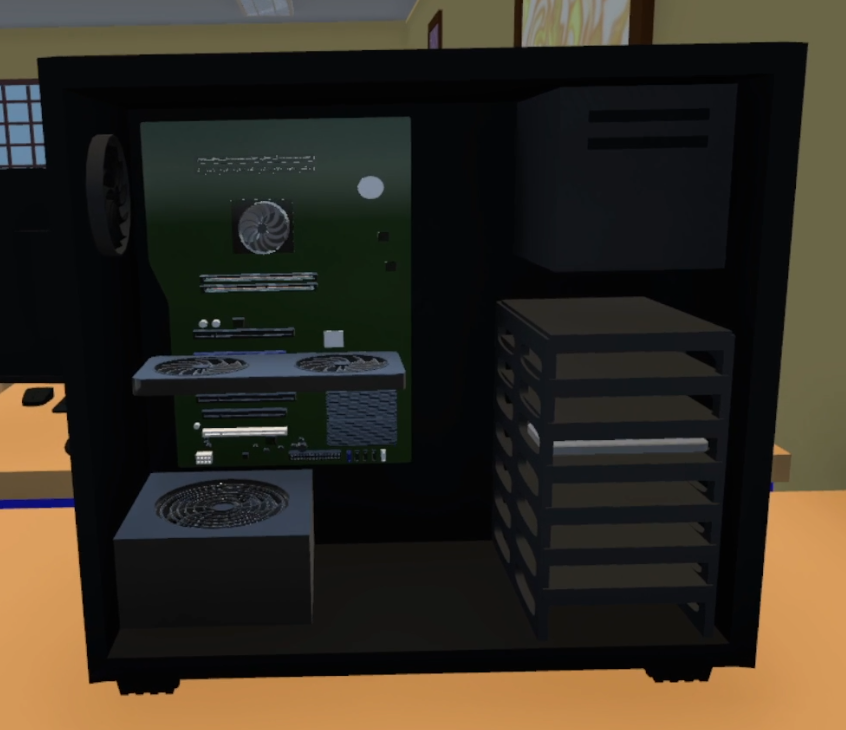
\includegraphics[width=0.6\textwidth]{image/pc.png} 
	\caption{Sestavený počítač ve virtuálním prostředí.} 
	\label{fig:pc} 
\end{figure}


\begin{figure}[H]
	\centering
	\subfloat{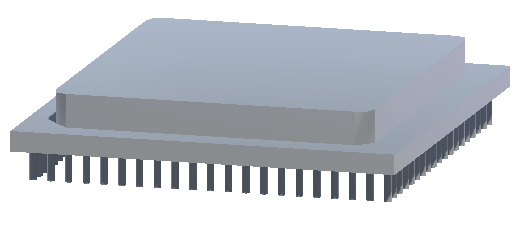
\includegraphics[width=7cm]{image/cpu.png}}
	\qquad
	\subfloat{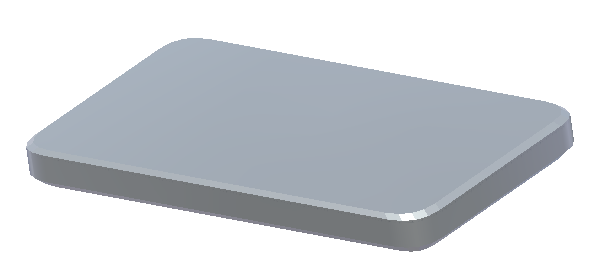
\includegraphics[width=7cm]{image/ssd.png}}
	\caption{Modely procesoru a SSD disku.}
	\label{fig:components}
\end{figure}

\begin{figure}[H]
	\centering
	\subfloat{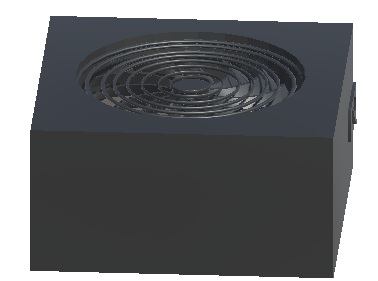
\includegraphics[width=7cm]{image/psu.png}}
	\qquad
	\subfloat{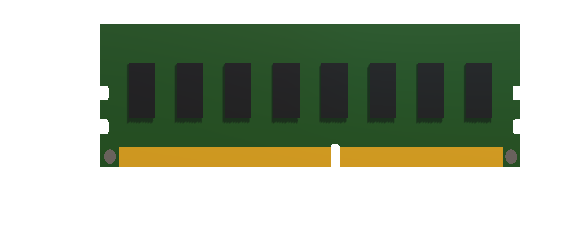
\includegraphics[width=7cm]{image/ram.png}}
	\caption{Modely zdroje počítače a paměti RAM.}
	\label{fig:components2}
\end{figure}

\begin{figure}[H]
	\centering 
	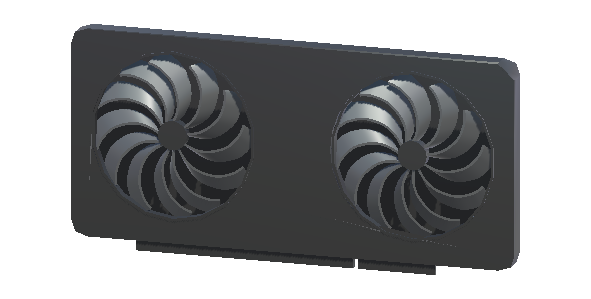
\includegraphics[width=0.6\textwidth]{image/gpu.png} 
	\caption{Model grafické karty.} 
	\label{fig:components3} 
\end{figure}
	
\chapter*{Závěr}
\addcontentsline{toc}{chapter}{Závěr}
Cílem projektu bylo pochopit problematiku virtuální reality a vytvořit aplikaci pro ní. Toho jsem dosáhl. Výsledkem práce je aplikace, která obsahuje interaktivní objekty, které lze vzít a házet. Dále obsahuje jednu třídu odborného předmětu, ve které lze sestavit počítač. Uživatel se ovládání a cíl místnosti může dozvědět z uživatelského menu na levé ruce.  
 
 Pochopil jsem problematiku virtuální reality a zlepšil jsem se v práci s herním enginem Unity. 
 
 Do budoucna bych chtěl určitě přidat více tříd a aktivit co v nich dělat. Také udělat menu pro výběr tříd nebo vytvořit halu, kde budou teleporty pro jednotlivé třídy.

Odkaz na projekt: \url{https://github.com/PandaLen/zaverecny-projekt}


%% Seznam použitých informačních zdrojů
\renewcommand\bibname{Seznam použitých informačních zdrojů}
\begin{thebibliography}{99}
\addcontentsline{toc}{chapter}{Seznam použitých informačních zdrojů}
\bibitem{VRGameTutorial} \textit{How to make a VR game - Unity XR Toolkit 2022} [online]. YouTube, 31.7.2023 [cit. 2024-01-13]. Dostupné z: \url{https://www.youtube.com/playlist?list=PLpEoiloH-4eP-OKItF8XNJ8y8e1asOJud}

\bibitem{ProBuilder} \textit{ProBuilder Building Structures with Interior and Exterior} [online]. YouTube, 6.3.2018 [cit. 2024-01-13]. Dostupné z: \url{https://www.youtube.com/watch?v=CBa_opm3_GM}	

\bibitem{ProBuilerTutorials}\textit{ProBuilder Unity Tutorials} [online]. YouTube, 27.8.2019 [cit. 2024-01-13]. Dostupné z: \url{https://www.youtube.com/playlist?list=PLs_yJ-RML1YeM2KbHbVKh50CkwINm-biV}

\bibitem{SnapZone} \textit{Introduction to VR in Unity - PART 8 : SNAP ZONE} [online]. YouTube, 23.7.2020 [cit. 2024-01-13]. Dostupné z: \url{https://www.youtube.com/watch?v=AWNhsSB6x9M}

\bibitem{HandMenu}\textit{How to make a Hand Menu - VR Tutorial} [online]. YouTube, 5.3.2023 [cit. 2024-01-13]. Dostupné z: \url{https://www.youtube.com/watch?v=6PSLfRsN89g}

\end{thebibliography}

%% obrázky 
\listoffigures



\end{document}